% Induction

\documentclass[12pt]{article}
\usepackage{graphicx}
\graphicspath{ {../art/} }

%%%%%%%%%%%%%%%%%%%%%%%%%%%%%%%%%%%%%%%%%%%%%%%%%%%%%%%%%%%%%%%%%
% Macros for formatting theorems, definitions, and proofs:
\newtheorem{theorem}{Theorem}[section]
\newtheorem{corollary}[theorem]{Corollary}
\newtheorem{lemma}[theorem]{Lemma}
\newtheorem{definition}{Definition}[section]
\def\proof{\rm \trivlist \item[\hskip \labelsep{\it Proof.}]}
\def\endproof{\hspace{1em}{\begin{picture}(6.5,6.5)%
  \put(0,0){\framebox(6.5,6.5){}}\end{picture}}\endtrivlist}

% Macros for formatting computer programs:
\newcommand{\id}[1]{\mbox{\it #1\/}}
\newcommand{\bid}[1]{\mbox{\bf #1}}
\newcommand{\tid}[1]{\mbox{\tt #1}}
\newcommand{\rid}[1]{\mbox{\rm #1}}
\newcommand{\query}{\mbox{$eq_h$}}
\newcommand{\whiledo}[2]{\mbox{\bf while ${#1}$ do ${#2}$}}
\newcommand{\ifthenelse}[3]{\mbox{\bf if ${#1}$ then ${#2}$ else ${#3}$}}
\newcommand{\ifthen}[2]{\mbox{\bf if ${#1}$ then ${#2}$}}

% Macros for formatting types:
% \txxx{#1} produces #1 xxx
\newcommand{\tvar}[1]{\mbox{${#1}\;\id{var}$}}
\newcommand{\tcmd}[1]{\mbox{${#1}\;\id{cmd}$}}

% Macros for sequential and global transitions and equivalence:
\newcommand{\Arrow}{\Rightarrow}
\newcommand{\strans}{\longrightarrow}
\newcommand{\gtrans}[1]{\mbox{$\stackrel{#1}{\longrightarrow}$}}
\newcommand{\equivgam}{\mbox{$\sim_{\gamma}$}}

% Names of evaluation rules:
\newcommand{\noop}{\mbox{\sc no-op}}
\newcommand{\update}{\mbox{\sc update}}
\newcommand{\sequence}{\mbox{\sc sequence}}
\newcommand{\branch}{\mbox{\sc branch}}
\newcommand{\loopr}{\mbox{\sc loop}}
\newcommand{\forloopr}{\mbox{\sc iterate}}

% Names of typing rules:
\newcommand{\conditional}{\mbox{\sc if}}
\newcommand{\while}{\mbox{\sc while}}
\newcommand{\base}{\mbox{\sc base}}
\newcommand{\reflex}{\mbox{\sc reflex}}
\newcommand{\cmdsub}{\mbox{\sc cmd$^-$}}
\newcommand{\subtype}{\mbox{\sc subtype}}

\newcommand{\prob}[1]{\mbox{Pr$[{#1}]$}}
\newcommand{\cprob}[2]{\mbox{Pr$[{#1}\mid{#2}]$}}
%%%%%%%%%%%%%%%%%%%%%%%%%%%%%%%%%%%%%%%%%%%%%%%%%%%%%%%%%%%%%%%%%

\begin{document}

\begin{flushleft}
{\huge {\bf Induction}}
\end{flushleft}

\vspace{7mm}
%\noindent Performed over a well-ordered set.

% both following lines uncommented: no page numbers anywhere
% second commented but not first: page numbers everywhere except first page
% first commented but not second: page number on first page only

\thispagestyle{empty}	
%\pagestyle{empty}	

\section{Weak Induction}

Suppose $S(n)$ is a statement involving variable $n$ which ranges over
values of a well-ordered set.
A weak induction rule is given below:
\begin{tabbing}
[1]XX \=  \kill
%[1] \>
	%\(\begin{array}[t]{l}
	%S(i) \;\wedge\; \forall n > i.\;S(n-1) \Rightarrow S(n) \\
	%\hline
	%\forall n \geq i. \; S(n)
	%\end{array}\) \\[2ex]
[1] \>
	\(\begin{array}[t]{l}
	S(i) \;\wedge\; \forall n \geq i.\;S(n) \Rightarrow S(n+1) \\
	\hline
	\forall n \geq i. \; S(n)
	\end{array}\) % \\[2ex]
\end{tabbing}
$S(i)$ is called the {\em basis\/} and $\forall n \geq i.\;S(n) \Rightarrow S(n+1)$
the {\em inductive step\/}.  % Both constitute the antecedent of the rule.

In showing the inductive step, you get to assume $S(n)$ is true where $n\geq i$.
The assumption is called the {\em inductive hypothesis\/}.
You DO NOT assume $S(n)$ is true for all $n\geq i$ as this is the conclusion of the rule
and would mean you're assuming what you're supposed to show!

\subsection{Examples of weak induction}

Let $S(n): \Sigma_{i=2}^{n}i = (n+2)(n-1)/2$.

\noindent Prove $S(n)$ by induction on $n$.
\[
\begin{array}[t]{l}
S(2) \,\wedge\, \forall n\geq 2.\, S(n)\Rightarrow S(n+1) \\
\hline
\forall n\geq 2.\, S(n)
\end{array}
\]
\noindent Basis: Show $S(2)$.

\noindent Inductive hypothesis: Suppose $S(n)$ {\bf where} $n\geq 2$.

\noindent Inductive step: Show $S(n+1)$.

\begin{proof}
\noindent Basis: Show $S(2): \Sigma_{i=2}^2 i = (2+2)(2-1)/2$, which is true.

\vspace{0.5em}
\noindent Inductive hypothesis: Suppose $S(n): \Sigma_{i=2}^{n}i = (n+2)(n-1)/2$ where $n \geq 2$.

\vspace{0.5em}
\noindent Inductive step: Show $S(n+1): \Sigma_{i=2}^{n+1} i = (n+3)n/2$.
\[\begin{array}{lll}
\Sigma_{i=2}^{n+1} i & = & \Sigma_{i=2}^n i + n + 1 \\
 & = & (n+2)(n-1)/2 + n + 1 \;\;\rid{by induction} \\
 & = & ((n+2)(n-1)+2n+2)/2 \\
 & = & (n^2 + n - 2 + 2n + 2)/2 \\
 & = & (n^2 + 3n)/2 \\
 & = & (n+3)n/2
\end{array}
\]
\end{proof}

Now let $S(n)$: if $x,y\in\Sigma^*$ and $|y|=n$ then $|xy| = |x| + n$.

\noindent Prove $S(n)$ by induction on $n$.
\[
\begin{array}[t]{l}
S(0)\,\wedge\,\forall n\geq 0.\, S(n)\Rightarrow S(n+1) \\
\hline
\forall n\geq 0.\, S(n)
\end{array}
\]
\noindent Basis: Show $S(0)$.

\noindent Inductive hypothesis: Suppose $S(n)$ {\bf where} $n\geq 0$.

\noindent Inductive step: Show $S(n+1)$.

\begin{proof}
\noindent Basis: Show $S(0)$: Suppose if $x,y\in\Sigma^*$ and $|y|=0$ then $|xy|=|x|+0$.
So suppose $x,y\in\Sigma^*$ and $|y|=0$.
Since $|y|=0$, $y=\epsilon$.  Thus $xy=x$. So it follows that $|xy|=|x|=|x| + 0$.

\vspace{0.5em}
\noindent Inductive hypothesis: Suppose $S(n)$: if $x,y\in\Sigma^*$ and $|y|=n$ then $|xy| = |x| + n$ {\bf where} $n\geq 0$.

\vspace{0.5em}
\noindent Inductive step: Show $S(n+1)$: if $x,y\in\Sigma^*$ and $|y|=n+1$ then $|xy| = |x| + n+1$.

\vspace{1em}
\noindent Suppose $x,y\in\Sigma^*$ and $|y|=n+1$.
Since $n\geq 0$, $n+1\geq 1$.
Therefore $y$ has the form $za$ where $z\in\Sigma^*$, $a\in\Sigma$ and $|z|=n$.
\[\begin{array}{lll}
|xy| & = & |x(za)| \\
 & = & |(xz)a| \;\;\rid{by associativity of string concatenation} \\
 & = & |xz| + 1 \\
 & = & |x|+n + 1 \;\;\rid{by induction}
\end{array}
\]
\end{proof}

\section{The need for strong induction}

Consider the following definition of expressions:

\[\begin{array}{ll}
{\bf B}. & a\in\id{Exp} \\[1ex]
{\bf R}. & \rid{if}\;e\in\id{Exp}\;\rid{then}\; \neg e\in\id{Exp}
\end{array}
\]
There is a basis {\bf B} and a recursive statement {\bf R}.
The recursive definition can be expressed as a Post System of inference rules as follows:
\begin{tabbing}
{\bf B}XX \=  \kill
{\bf B} \>
	\(\begin{array}[t]{l}
	a\in\id{Exp} 
	\end{array}\) \\[2ex]
{\bf R} \>
	\(\begin{array}[t]{l}
	e\in\id{Exp} \\
	\hline
	\neg e\in\id{Exp}
	\end{array}\) % \\[2ex]
\end{tabbing}
Rule {\bf B} has no antecedent or premise for
``a'' to be an expression.
Hence it is an {\em axiom\/}.
Rule {\bf R} requires $e$ to be an expression if $\neg e$ is to be one.

Proofs are {\em derivations\/}.
For example, $a\in\id{Exp}$ has a derivation or proof:
\begin{center}
\begin{tabular}{ll}
$\bid{B}$ & $a\in\id{Exp}$
\end{tabular}
\end{center}
It has height zero.  Likewise, $\neg\neg a\in\id{Exp}$ has a derivation but of height 2:
\begin{center}
\begin{tabular}{ll}
$\bid{B}$ & $a\in\id{Exp}$ \\ \cline{2-2}
$\bid{R}$ & $\neg a\in\id{Exp}$ \\ \cline{2-2}
$\bid{R}$ & $\neg\neg a\in\id{Exp}$ 
\end{tabular}
\end{center}

Now suppose we wish to prove that whenever we can derive $e\in\id{Exp}$ then
every subexpression of $e$ contains ``a''.
This can be done by a {\em weak\/} induction on the height of the derivation of $e\in\id{Exp}$
as follows.

\begin{proof}
\noindent {\em Basis\/}:
derivation height is zero.
There's only one derivation of height zero and it's for $a\in\id{Exp}$.  
Clearly ``a'' contains ``a''.

\noindent {\em Inductive step\/}:
Suppose $n\geq 0$ and if $e\in\id{Exp}$ has derivation height $n$ then every
subexpression of $e$ contains ``a''.
Show if $e'\in\id{Exp}$ has derivation height $n+1$, where $n\geq 0$,
then every subexpression of $e'$ contains ``a''.

Since $n\geq 0$, $n+1\geq 1$.
Thus the derivation height of $e'\in\id{Exp}$ is at least 1 which implies the derivation must end
with an application of rule {\bf R}:
\begin{center}
\begin{tabular}{ll}
 & $e\in\id{Exp}$ \\ \cline{2-2}
$\bid{R}$ & $\neg e\in\id{Exp}$ 
\end{tabular}
\end{center}
where $e' = \neg e$.
The derivation of $e\in\id{Exp}$ must have height $n$ since the derivation of $e'\in\id{Exp}$ has height $n+1$.
Therefore by the inductive hypothesis, every subexpression of $e$ contains ``a''.
And since $e$ is the only subexpression of $\neg e$, every subexpression of $e'$ contains ``a''.
\end{proof}

Now suppose we extend our definition of expressions to include sum:
\begin{tabbing}
{\bf R2}XX \=  \kill
{\bf B} \>
	\(\begin{array}[t]{l}
	a\in\id{Exp}
	\end{array}\) \\[2ex]
{\bf R1} \>
	\(\begin{array}[t]{l}
	e\in\id{Exp} \\
	\hline
	\neg e\in\id{Exp}
	\end{array}\) \\[2ex]
{\bf R2} \>
	\(\begin{array}[t]{l}
	e_1\in\id{Exp}\;\;\;e_2\in\id{Exp} \\
	\hline
	e_1 + e_2\in\id{Exp}
	\end{array}\) % \\[2ex]
\end{tabbing}
Suppose we again try to prove that $e\in\id{Exp}$ implies every subexpression of $e$ contains ``a''.
In the inductive step, we now have two cases:
the derivation of $e'\in\id{Exp}$ ends with {\bf R1} or it ends with an application of {\bf R2}:
\begin{center}
\begin{tabular}{ll}
 & $e_1\in\id{Exp}\;\;\; e_2\in\id{Exp}$ \\ \cline{2-2}
$\bid{R2}$ & $e_1+e_2\in\id{Exp}$ 
\end{tabular}
\end{center}
where $e' = e_1 + e_2$.
We know $e'\in\id{Exp}$ has derivation height $n+1$ so $e_1\in\id{Exp}$ or $e_2\in\id{Exp}$ 
has derivation height $n$.
The other though may have height less than $n$.
For instance, $e_1$ may be $a+a$ while $e_2$ is just $a$:
\begin{center}
\begin{tabular}{llll}
$\bid{B}$ & $a\in\id{Exp}$ & $\bid{B}\;\;\;a\in\id{Exp}$ \\ \cline{2-3}
$\bid{R2}$ & \multicolumn{2}{c}{$a+a\in\id{Exp}$} & $\bid{B}\;\;\;a\in\id{Exp}$ \\ \cline{2-4}
$\bid{R2}$ & \multicolumn{3}{c}{$a+a+a\in\id{Exp}$} 
\end{tabular}
\end{center}
The derivation of $e_1+e_2\in\id{Exp}$ has height 2, 
the derivation of $e_1\in\id{Exp}$ has height 1 and the derivation of
$e_2\in\id{Exp}$ has height zero.
But the weak inductive hypothesis applies only to the derivation of height $1$!

For this reason, we must use a {\em strong\/} inductive hypothesis:

\begin{quote}
Suppose for all $k$ where $0\leq k\leq n$ and $n\geq 0$,
every subexpression of $e$ contains ``a'' if $e\in\id{Exp}$ has derivation height $k$.
\end{quote}

\subsection{Strong induction single base case}

The strong induction rule with a single base case is given below:
\begin{tabbing}
[2]XX \=  \kill
[2] \>
	\(\begin{array}[t]{l}
	S(i) \;\wedge\; \forall n \geq i.\;S(i)\;\wedge\;S(i+1)\;\wedge\cdots\wedge\;S(n) \Rightarrow S(n+1) \\
	\hline
	\forall n \geq i. \; S(n)
	\end{array}\)
\end{tabbing}
The induction rule is strong because you get to assume
$S(i)$, $S(i+1)$ through $S(n)$ are true when establishing $S(n+1)$ where $n\geq i$.

\subsection{Another example of strong induction}

\noindent A {\em tree\/} is an undirected acyclic connected graph.
See example in Fig.\ \ref{sp}.

\begin{figure}[h]
\centering
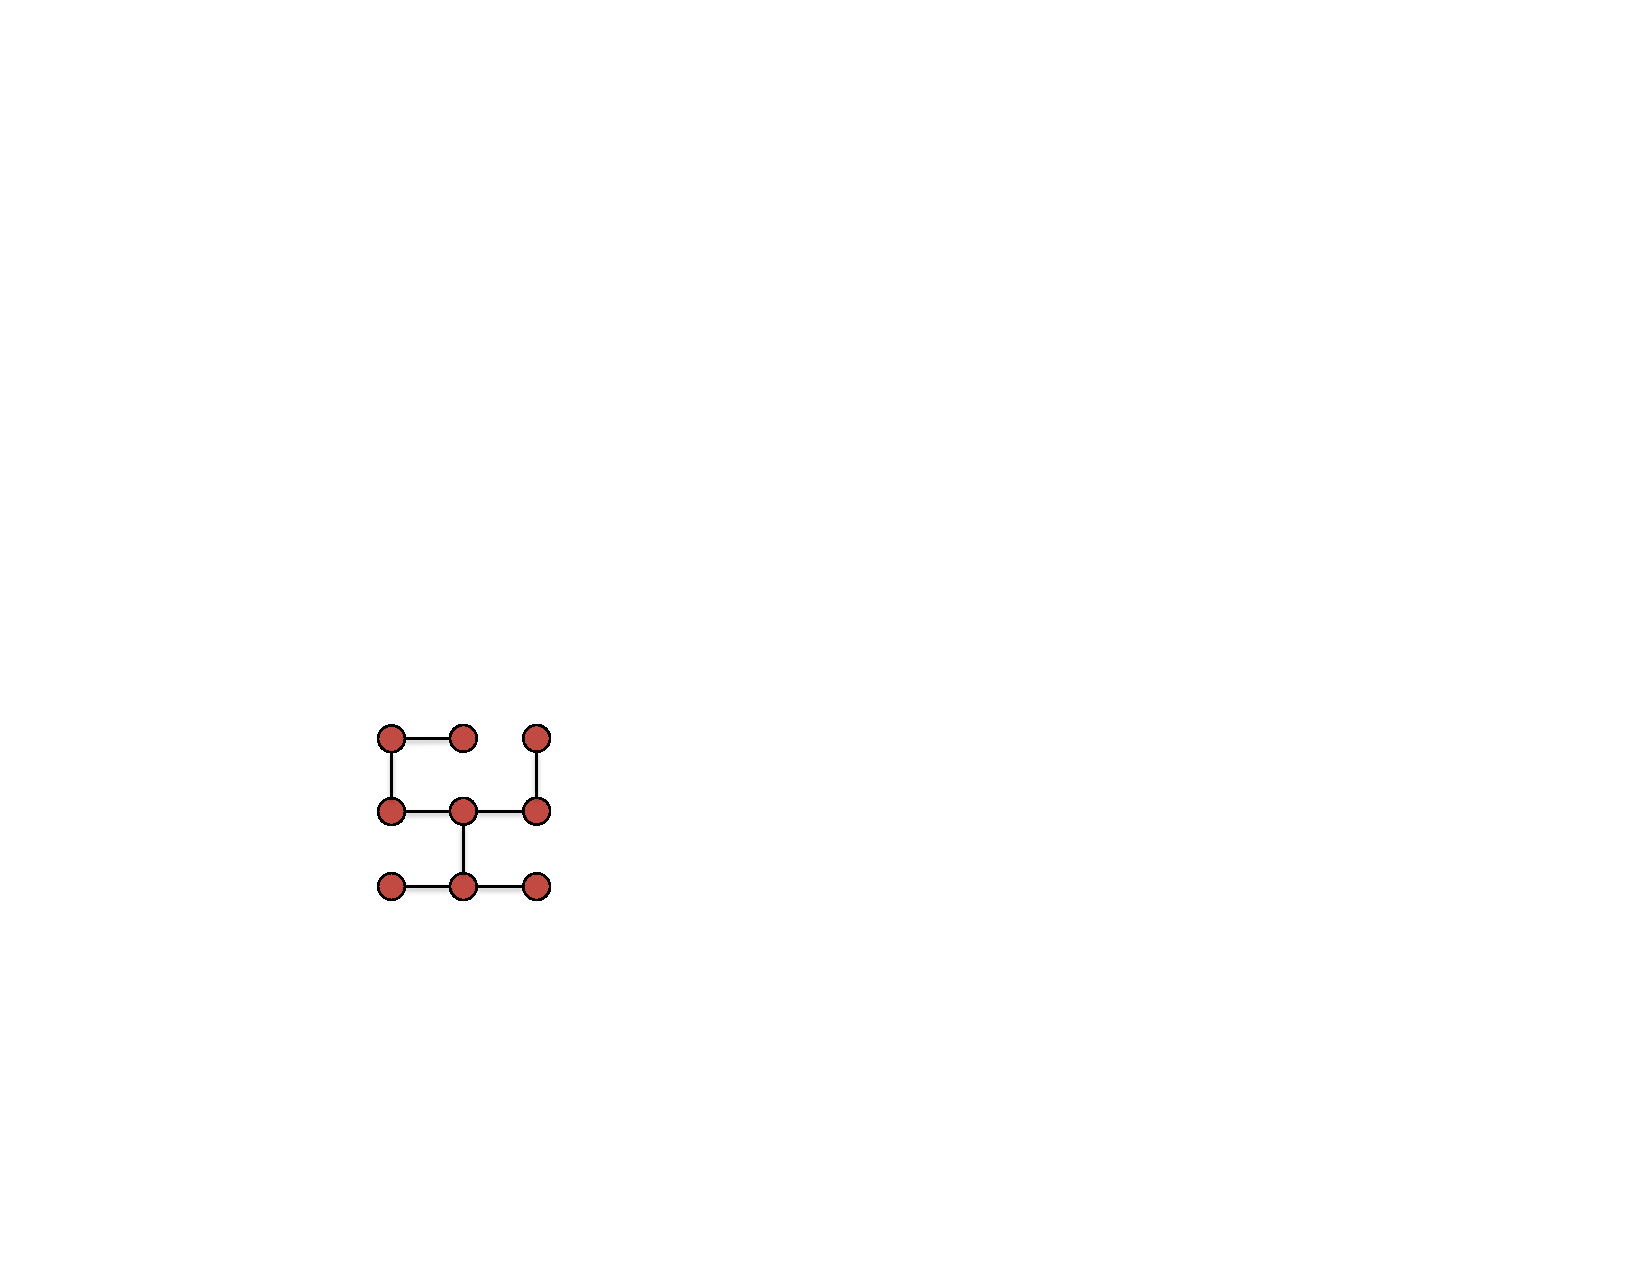
\includegraphics[width=1.5in, height=1.5in,keepaspectratio=true]{tree.pdf}
\caption{An example of a tree}
\label{sp}
\end{figure}

\vspace{0.5em}

\noindent Removing an edge from a tree with $n$ nodes yields two trees, each 
having fewer nodes but not necessarily $n-1$.

\vspace{0.5em}
\noindent For instance, removing an edge from the tree in Fig.\ \ref{sp} having 9 nodes can yield 
two trees with 3 and 6 nodes or two trees with 1 and 8 nodes (see Fig.~\ref{2sp}).
An induction on $n$ must therefore be strong so that its inductive hypothesis
covers all these cases when an edge is removed.

\begin{figure}[h]
\centering
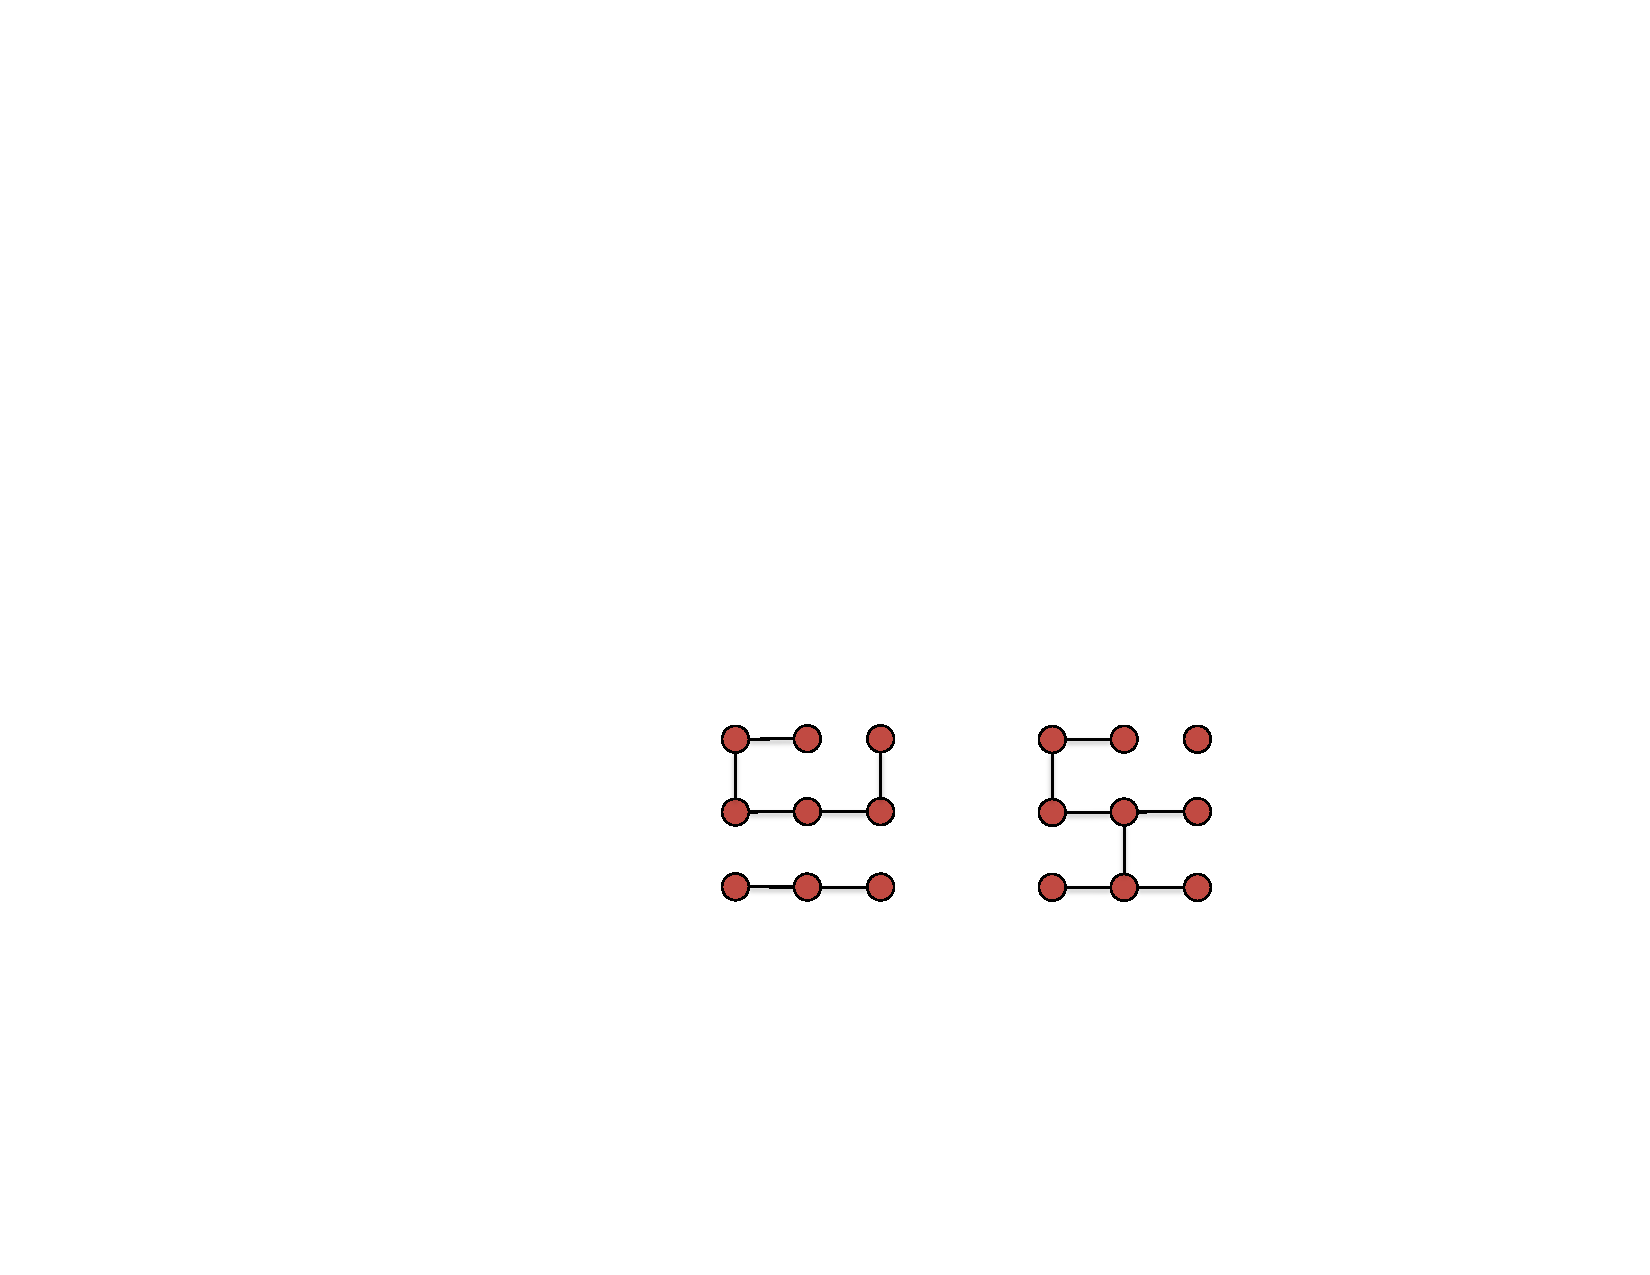
\includegraphics[width=3.5in, height=1.5in,keepaspectratio=true]{deletededge.pdf}
\caption{Deleting a different edge from the tree in Fig.\ref{sp}}
\label{2sp}
\end{figure}

\noindent {\bf Theorem}. If $(V,E)$ is a tree then $|E| = |V| - 1$.

\begin{proof}
The proof is by induction on $|V|$.
It is a strong induction.

\noindent{\em Basis\/}. $|V|=1$.  Since $(V,E)$ is a tree, it is acyclic.
Therefore $E$ is empty since $|V|=1$.  Thus $|E|=0=|V|-1$.

\noindent {\em Inductive step\/}.
Suppose $n>1$ and for all $1\leq k < n$, a tree with $k$ vertices has $k-1$ edges.
Show that a tree $(V',E')$ with $n$ vertices has $n-1$ edges.

Since $(V',E')$ is a tree, removing an edge $e\in E'$ leaves two trees
$(V_1,E_1)$ and $(V_2,E_2)$ such that $V'=V_1\cup V_2$, $V_1\cap V_2=\emptyset$ and
$E' = E_1\cup E_2\cup\{e\}$.
Since $1\leq |V_1| < n$, $|E_1|= |V_1|-1$ by induction.
Likewise, $1\leq |V_2| < n$ so $|E_2| = |V_2|-1$ by induction.
Therefore, $|E'| = |V_1| - 1 + |V_2| - 1 + 1$ which is $|V'|-1$ or $n-1$.
\end{proof}

\subsection{Strong induction multiple base cases}
\begin{tabbing}
[3]XX \=  \kill
[3] \>
	\(\begin{array}[t]{l}
	S(i) \;\wedge\; S(i+1)\;\wedge\cdots\wedge\;S(j)\;\wedge\; \\
\forall n \geq j.\;S(i)\;\wedge\;S(i+1)\;\wedge\cdots\wedge\;S(n) \Rightarrow S(n+1) \\
	\hline
	\forall n \geq i. \; S(n)
	\end{array}\) % \\[2ex]
\end{tabbing}
The induction rule is strong because you get to assume
$S(i)$, $S(i+1)$ through $S(n)$ are true when establishing $S(n+1)$ where $n\geq j$.
%See Example 1.18 of the textbook for an instance of this rule.

As a general rule, whenever a derivation of any kind permits more than one subderivation then
induction on derivation length calls for strong induction since some subderivations can be
much shorter in length than the length of the derivation minus 1.  
%See sidebar on page 181 of the textbook.

\section{Structural induction}

\begin{itemize}
\item  Induction over the size of a data structure.
Basically, it's a special case of induction on derivation height.

\item Terms in antecedent have smaller size than those in the consequent.

\item May be weak or strong.
For instance, the proof that every subexpression of an expression defined by rules {\bf B} and {\bf R}
contains ``a'' is a {\em weak\/} structural induction whereas the proof of this statement for
rules {\bf B}, {\bf R1} and {\bf R2} is a {\em strong\/} structural induction.
%Examples 1.19 and 1.20 of the textbook are both examples of strong structural induction.

\item So what's the advantage of structural induction?
It allows one to do induction over the size of a structure or term, so there's no
need to introduce a Post system and do induction on derivation height.

\item Keep in mind that induction on derivation height is more general because
it does not require terms in every antecedent to have smaller size than terms in the consequent.
\end{itemize}

\section{Mutual induction}

\begin{itemize}

\item Just a way to organize a proof by induction on $n$ of the statement $S_1(n)\wedge\cdots\wedge S_k(n)$.

\item May be weak or strong.

\item Weak version is often used to prove properties of finite state systems.
\end{itemize}
\end{document}
